\documentclass{article}
\title{Metodologia para escolha de sensores infravermelho para atuação em duas aplicações distintas}
\date{}

\usepackage[utf8]{inputenc}
\usepackage[portuguese]{babel}
\usepackage[margin=3.5cm]{geometry}
\usepackage{amsmath}
\usepackage{physics}
\usepackage{titlesec}
\usepackage{graphicx}
\usepackage{wrapfig}
\usepackage{caption}
\usepackage{subcaption}
\usepackage[parfill]{parskip}
\usepackage[nottoc]{tocbibind}
\usepackage[backend=biber]{biblatex}
\addbibresource{/home/luispengler/drive/LinuxFabrik/Research/read/bib.bib}
\usepackage{authblk}
\author[1]{Luís Spengler}
\affil[1]{Instituto Federal de Educação, Ciência e Tecnologia de Mato Grosso do Sul}

\begin{document}
\maketitle

\section{Introdução}
Sensores fotoelétricos são usados para detectar a presença ou ausência de um objeto dentro de uma área delimitada, emitindo luz visível ou infravermelha. 
Nesse sentido, se torna viável a utilização de sensores para projetos de automação que uma das variáveis seja a presença ou ausência de algo.

Este presente artigo foca em determinar o melhor sensor dentre os infravermelho para identificar a passagem de ouro em uma linha de trituração e o melhor entre os dois para identificar se há um objeto qualquer passando em uma linha de produção.
\section{Problemática}
Minas de ouro e produção de produtos quaisquiser são dois ambientes distintos, mas ambos podem se beneficiar da instrumentação e controle para redução de gastos. A primeira, pois o lucro não vem se não for achado o ouro, tornando-se necessário métodos de detecção de ouro entre rochas em uma esteira presente em uma linha de trituração. E o outro, evitar gastos desnecessários quando quaisquiser produtos em uma linha de produção não estão sendo locomovidos por uma esteira.

\section{Objetivo Geral}
Determinar o sensor de temperatura infravermelho mais adequado para detecção de metais (ouro) e o mais adequado na identificação de um objeto qualquer em uma linha de produção, almejando máximização do lucro e redução de custos.

\section{Metodologia}
Para este presente estudo vamos analisar dois tipos de sensores infravermelho: retroreflector e difuso. Vamos primeiro analisar os retroreflectores. Existem dois tipos, aqueles que emitem ondas polarizadas e os que não. Não polarizados não saberiam diferenciar o seu espelho retro-refletor de um objeto metálico, se este redirecionasse o feixe do emissor diretamente no receptor. Neste caso, objetos metálicos, às vezes, fariam o nível lógico voltar pra 0. Com objetos normais, o nível lógico continuaria sendo 1. É sensível até 7m. No entanto, para o tipo de ondas polarizadas, qualquer objeto que interrompa o feixe, mesmo que este seja metálico (ou até outro espelho), o sinal lógico continua sendo 1 e é sensível de 3 a 5,5m. 

Agora vamos analisar o sensor difuso. A diferença entre este e o retroreflector, é que usam o alvo para mandar a luz de volta (em vez de um espelho). No entanto, nem todos os alvos são bons em emitir luz de volta e precisam estar mais perto do que alguns para serem detectados. Sensores de proximidade difusos tem um alcance de até 500mm. Qualquer alvo dentro deste alcance vai ser visto, contanto que reflita luz suficiente. 
Basta, portanto, entender as características dos objetos analisados nas duas linhas de máquinas e teremos nossa resposta para o mais adequado.

%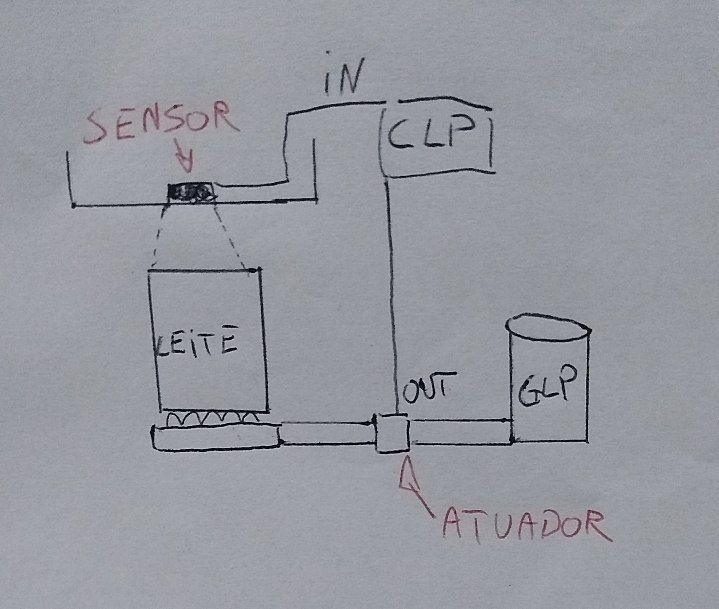
\includegraphics[scale=0.3]{esquema}

\section{Resultados}
Com as características dos dois tipos de sensores abordados, vamos nos voltar para a aplicação da linha de trituração. É possível que para alguns, apenas a utilização de sensores retroreflectores não polarizados seja capaz de resolver o problema proposto. No entanto, vamos nos voltar mais uma vez para a aplicação do sensor difuso e veremos que este pode ser mais prático, pois qualquer alvo que reflita luz suficiente para ser detectado, vai mudar o sinal lógico de 0 para 1. Bastando, então, posicionarmos o sensor longe o suficiente para os materiais mais comuns dessa linha de produção não "triggarem" o sensor, i.e. mudarem o sinal lógico de 0 para 1.

Nos voltando para a aplicação da linha de produção, que desliga se por um tempo maior do que 10 segundos apresentar um nível lógico baixo, fica claro que o mais eficiente seria um sensor retroreflector de luz polarizada. Não importando o objeto que passasse na sua área de detecção, este sempre apresentaria nível lógico 1. Não havendo nenhum objeto, o sinal lógico torna-se 0 e por um tempo maior do que 10 segundos, a esteira desliga.
\section{Conclusão}
Determinamos que para aplicações que envolvem distinção de um objeto metálico de foscos, viz. linha de trituração de uma mina de ouro, um sensor difuso seria mais adequado. Para uma aplicação que não importando o tipo de material, um sensor retroreflector polarizado seria mais adequado.

\subsection{Adendo}
Sensores de proximidade capacitivos e indutivos não operam na frequência infravermelha, mas estes ainda poderiam ser utilizados na aplicação da linha de produção e linha de trituração com as seguites condições. 

Sensores de proximidade capacitivos seriam mais adequados para a linha de produção, pois pode-se ativar o nível lógico alto deste sensor com praticamente qualquer material. Metais, todos os tipos de plástico, madeira, papel, vidro, tecido e até mesmo liquidos em recepiente não metálicos. Este tipo de sensor se torna tão preciso quanto o sensor retroreflector não polarizado, para a mesma aplicação.

Sensores de proximidade indutivos teoricamente funcionariam com péssimo desempenho na aplicação da linha de trituração, onde deve-se atentar à passagem de ouro. Esse tipo de sensor funciona com sua maior range em objetos ferrosos e vai diminuindo de acordo com a quantidade de ferro que um material possui. Ouro pode até se fazer detectável por este sensor, mas sua range terá que ser diminuída de acordo com o datasheet do modelo do sensor. Este tipo de sensor se torna menos viável que o difuso para a mesma aplicação.

\end{document}
